\subsection{Results Affine Registration}
The dice after the affine registration can be seen in ~\ref{fig:result_affine}. It shows the three dices for 936 different parameter combinations tested on ten patients. The registration took approximatly 15.0 seconds with a standard deviation of 10.6. The mean of the grey matter is 0.50 and a standard deviation of 0.02, for the ventricles it is 0.47 $\pm$ 0.09, and for the white matter the mean is 0.62 and a standard deviation of 0.02. The results of the ventricles have the highest range, with a dice spanning from 0.04 to 0.65.

\begin{figure}[!h]
	\centering
	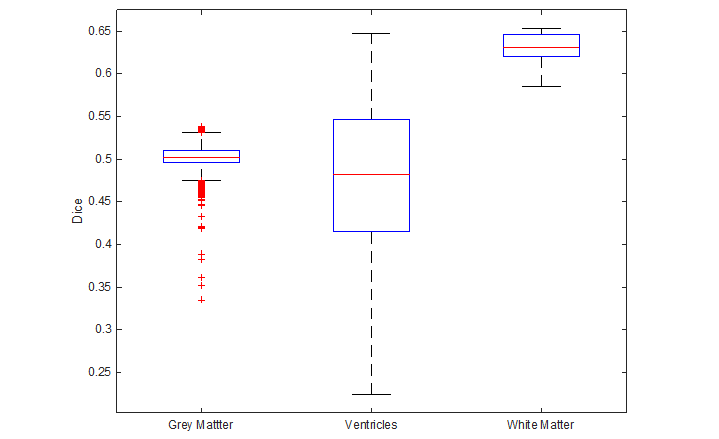
\includegraphics[width=4in]{results_affine}
	% where an .eps filename suffix will be assumed under latex, 
	% and a .pdf suffix will be assumed for pdflatex; or what has been declared
	% via \DeclareGraphicsExtensions.
	\caption{The boxplot of the dice after the registration.}
	\label{fig:result_affine}
\end{figure}